\documentclass[10pt,twocolumn,hidelinks,letterpaper]{article}

\usepackage[table]{xcolor}
\usepackage{cvpr}
\usepackage{times}
\usepackage{epsfig}
\usepackage{graphicx}
\usepackage{amsmath}
\usepackage{amssymb}

\usepackage[utf8x]{inputenc}
\usepackage[english]{babel}
\usepackage{url}
\usepackage{lipsum}

\usepackage[framed , numbered]{matlab-prettifier}
\usepackage{listings}
\usepackage{setspace}
\usepackage{color} %red, green, blue, yellow, cyan, magenta, black, white
\usepackage{geometry}
\usepackage{subcaption}
\usepackage{graphicx}
\usepackage{float}


% Include other packages here, before hyperref.

% If you comment hyperref and then uncomment it, you should delete
% egpaper.aux before re-running latex.  (Or just hit 'q' on the first latex
% run, let it finish, and you should be clear).
\usepackage[breaklinks=true,bookmarks=false]{hyperref}

\cvprfinalcopy % *** Uncomment this line for the final submission

\def\cvprPaperID{****} % *** Enter the CVPR Paper ID here
\def\httilde{\mbox{\tt\raisebox{-.5ex}{\symbol{126}}}}

% Pages are numbered in submission mode, and unnumbered in camera-ready
%\ifcvprfinal\pagestyle{empty}\fi
\setcounter{page}{1}
\begin{document}

%%%%%%%%% TITLE
\title{01TXFSM - Machine Learning and Deep Learning \\
\vspace{0.3in}
Final Project \\
First Person Action Recognition}

\author{
  Eros Fanì - s269781\\
  Politecnico di Torino\\
  {\tt\small eros.fani@studenti.polito.it}
  \and
  Gabriele Trivigno - s276807\\
  Politecnico di Torino\\
  {\tt\small gabriele.trivigno@studenti.polito.it}
  \and
  Cristiano Gerbino - s277058\\
  Politecnico di Torino\\
  {\tt\small s277058@studenti.polito.it}
}

\maketitle
%\thispagestyle{empty}

\lstset{language=python,%
  %basicstyle=\color{red},
  breaklines=true,%
  morekeywords={matlab2tikz},
  keywordstyle={\small \color{blue}},%
  morekeywords=[2]{1}, keywordstyle=[2]{\small \color{black}},
  identifierstyle={\small \color{black}},%
  stringstyle={\small \color{mylilas}},
  commentstyle={\small \color{mygreen}},%
  showstringspaces=false,%without this there will be a symbol in the places where there is a space
  numbers=left,%
  numberstyle={\small \color{black}},% size of the numbers
  numbersep=7pt, % this defines how far the numbers are from the text
  emph=[1]{error,warning},emphstyle=[1]{\small \color{red}} %some words to emphasise
  %emph=[2]{word1,word2}, emphstyle=[2]{style},
}

%%%%%%%%% BODY TEXT
\newcommand{\quotes}[1]{“#1”}
\newcommand{\reff}[1]{Figure \ref{#1}}
\setlength{\parindent}{0pt}
\setstretch{0.1}
\setlength{\parskip}{1em}
\definecolor{TopRow}{HTML}{E6E6FF}

\begin{abstract}


\end{abstract}

\section{Introduction}

\subsection{Goals}

The first goal of the project is to replicate some of the experiments performed in \cite{egornn} and \cite{sparnet}. The objective of these studies is the First Person Action Recognition: they tried to implement a deep learning model capable to extract meaningful features to automatically predict the action filmed by a wearable camera.

After having replicated these experiments we performed a grid search on the experiments to find the best set of values for the hyperparameters.

At last we have tried to improve the performances of the results of \cite{egornn} and \cite{sparnet} with some innovative ideas.

\subsection{Our contribution}

\[...\]

\subsection{Data exploration}

The dataset under analysis is a modified version of GTEA61\footnote{Georgia Tech Egocentric Activity Datasets: \small{\url{http://cbs.ic.gatech.edu/fpv/}}}. The dataset contains the videos in form of frames, and also two kind of preprocessed images: \textit{motion maps} and \textit{optical flows}. The folder schema of the dataset is shown in \reff{folder_schema}. Videos represent 61 class actions performed by 4 different users (\textit{S1}, \textit{S2}, \textit{S3}, \textit{S4}). Sometimes for some actions more than one video is available. The total number of videos in the dataset is, however, 457, which actually means that it is a quite small dataset.

\begin{figure*}
	\centering
	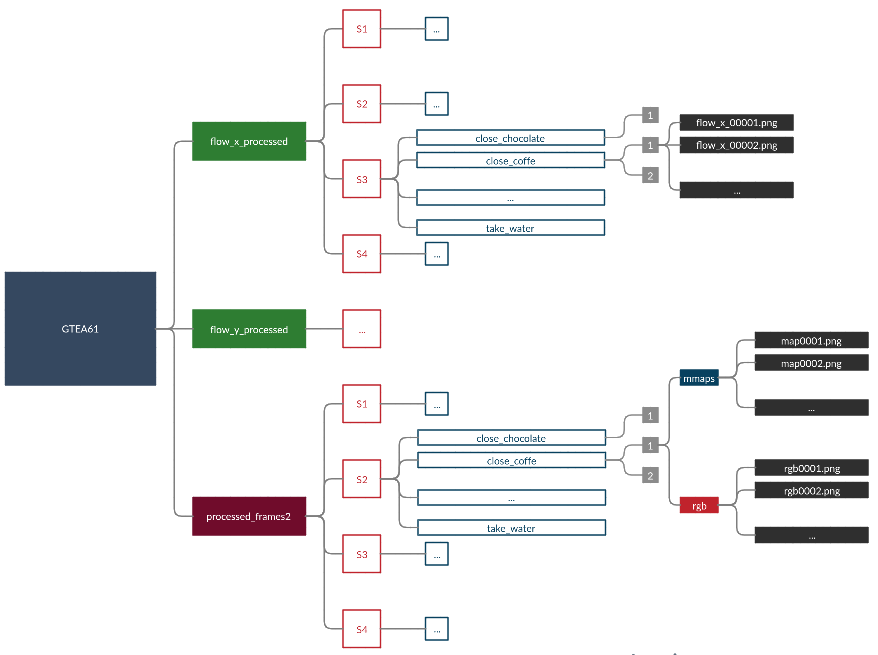
\includegraphics[width=.9\linewidth]{images/folder_schema.png}
	\caption{Folder schema of our GTEA61}
	\label{folder_schema}
\end{figure*}

The optical flow methods try to calculate the motion between two image frames which are taken at times $t$ and $t + \Delta t$ at every voxel position. The warp flow methods try also to remove the motion of the wearable camera. We have two kind of these last representations in our dataset: one computed in the horizontal axis (folder \textit{flow\_x\_processed}) and one other computed in the vertical axis (folder \textit{flow\_y\_processed}).

The motion maps are special black-and-white images which represent the spatial location in which the Motion Segmentation task of \cite{sparnet} focuses its attention per each frame. The mmaps present large similarities with the warp flows.

The differences between the kind of available images in our dataset are shown in \reff{image_comparison}.

\begin{figure*}
  \centering
  \begin{subfigure}{.24\linewidth}
  	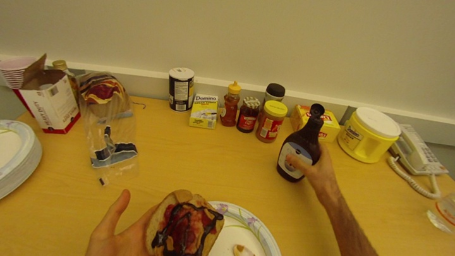
\includegraphics[width=\linewidth]{images/img_comp/rgb0001.png}
  \end{subfigure}
  \begin{subfigure}{.24\linewidth}
  	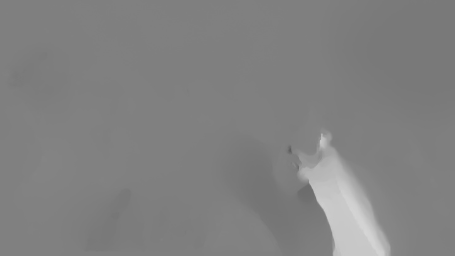
\includegraphics[width=\linewidth]{images/img_comp/flow_x_00002.png}
  \end{subfigure}
  \begin{subfigure}{.24\linewidth}
  	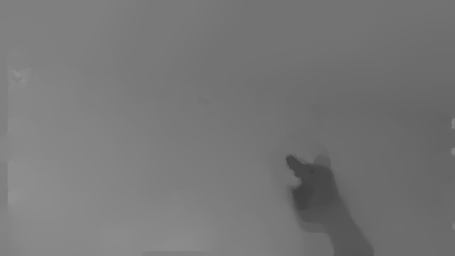
\includegraphics[width=\linewidth]{images/img_comp/flow_y_00001.png}
  \end{subfigure}
  \begin{subfigure}{.24\linewidth}
  	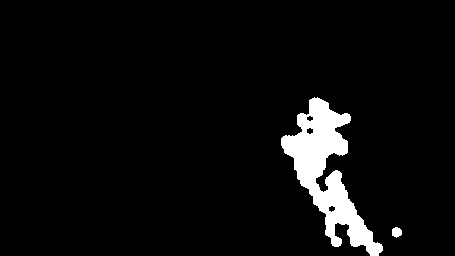
\includegraphics[width=\linewidth]{images/img_comp/map0001.png}
  \end{subfigure}
  \begin{subfigure}{.24\linewidth}
  	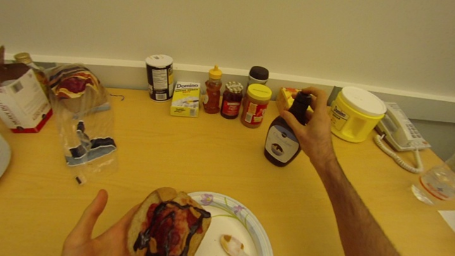
\includegraphics[width=\linewidth]{images/img_comp/rgb0011.png}
  \end{subfigure}
  \begin{subfigure}{.24\linewidth}
  	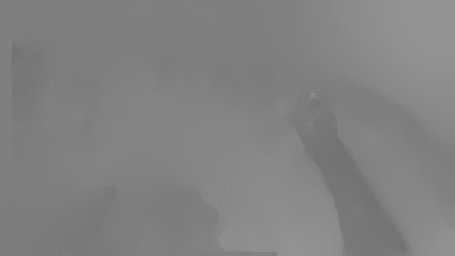
\includegraphics[width=\linewidth]{images/img_comp/flow_x_00011.png}
  \end{subfigure}
  \begin{subfigure}{.24\linewidth}
  	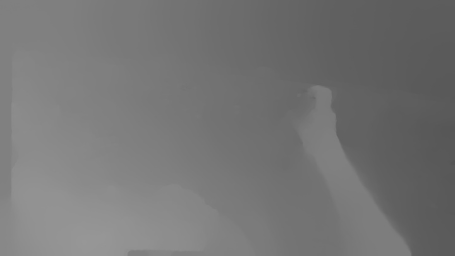
\includegraphics[width=\linewidth]{images/img_comp/flow_y_00011.png}
  \end{subfigure}
  \begin{subfigure}{.24\linewidth}
  	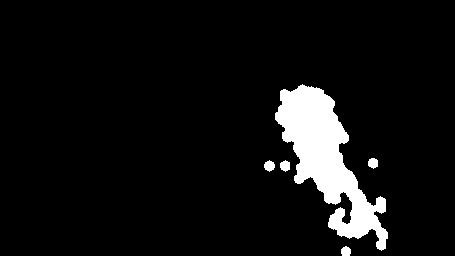
\includegraphics[width=\linewidth]{images/img_comp/map0011.png}
  \end{subfigure}
  \begin{subfigure}{.24\linewidth}
  	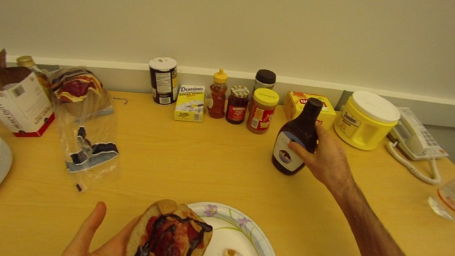
\includegraphics[width=\linewidth]{images/img_comp/rgb0020.png}
  \end{subfigure}
  \begin{subfigure}{.24\linewidth}
  	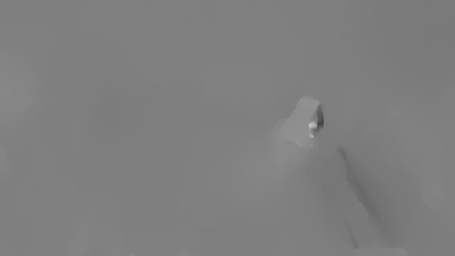
\includegraphics[width=\linewidth]{images/img_comp/flow_x_00020.png}
  \end{subfigure}
  \begin{subfigure}{.24\linewidth}
  	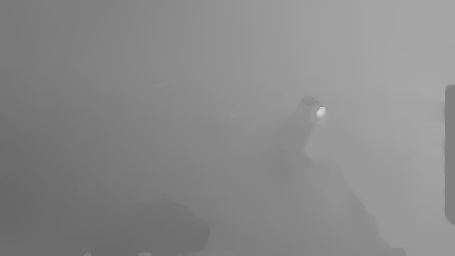
\includegraphics[width=\linewidth]{images/img_comp/flow_y_00020.png}
  \end{subfigure}
  \begin{subfigure}{.24\linewidth}
  	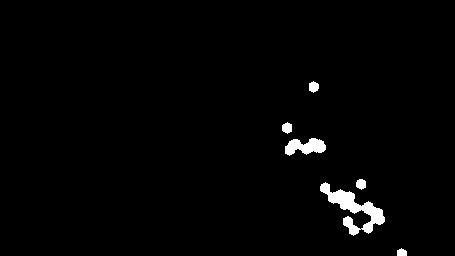
\includegraphics[width=\linewidth]{images/img_comp/map0020.png}
  \end{subfigure}
  \caption{Types of images in our dataset. In this example is shown a sample of images from the \textit{close\_chocolate} action. From the left column to the right column: rgbs, warp flows x, warp flows y, motion maps}
  \label{image_comparison}
\end{figure*}

\subsection{Data cleaning}

The dataset was almost clean already from the beginning, but we encountered two problems within it:
\begin{itemize}
  \item there were hidden useless folders \textit{.DSstore} inside each one of the user folders. These have been removed
  \item some of the first mmaps of some videos were missing. In these cases we have simply duplicated the second mmap
\end{itemize}

\section{Descriptions of the models}

Here we describe the models that we have used to perform our experiments.

\subsection{Egornn}

Egornn is a Recurrent Neural Network. The overall architecture of \textit{egornn} is shown in \reff{egornn_arch}. This net is based on \textit{resnet34}\cite{resnet}, which constitutes the main block. \textit{resnet34} has five convolutional layers inside itself: with respect to \reff{egornn_arch} they are: \textit{Conv}, \textit{Layer1}, \textit{Layer2}, \textit{Layer3} and , \textit{Layer4}. From now on we'll call these blocks respectively \textit{conv1}, \textit{conv2}, \textit{conv3}, \textit{conv4} and \textit{conv5}.

At the termination of the \textit{resnet34} is placed a \textit{Spatial Attention Layer}. It includes a \textit{Class Activation Map} (CAM) that is capable to identify the image regions that have been used by the CNN to identify the class under analysis. It is computed by taking the output of the \textit{softmax} layer and the output of \textit{conv5} and taking the linear combination of all the weights of \textit{conv5} and the weights of the softmax.

% We can graphically see some of our CAMs in \reff{cams}.
%%% ADD CAMS %%%

The output of the CAM is then sent to a \textit{softmax} layer to obtain a probability map, which is called \textit{Spatial Attention Layer} (SAM). The output of the SAM is finally multiplied, cell by cell (Hadamard product), with the output of \textit{conv5}, obtaining another tensor of weights which is sent to a \textit{Convolutional Long Term Support Memory} block (ConvLSTM).

The reason for the usage of the ConvLSTM block is that, up to now, what the net does is to take each frame and to try to make predictions based only on the features that the net can extract from those frames, without taking into consideration the temporal encoding of frame level features. The convLSTM block take into consideration, for each frame $i$, both the output of the SAM for the layer i and the output of the ConvLSTM for the layer $i-1$, constituting a recursive structure.

The last output of the ConvLSTM (the output obtained from the last frame of a particular video) is average pooled and reshaped to obtain a final classification layer with 61 neurons (i.e. the number of classes of our dataset).

\begin{figure*}
	\centering
	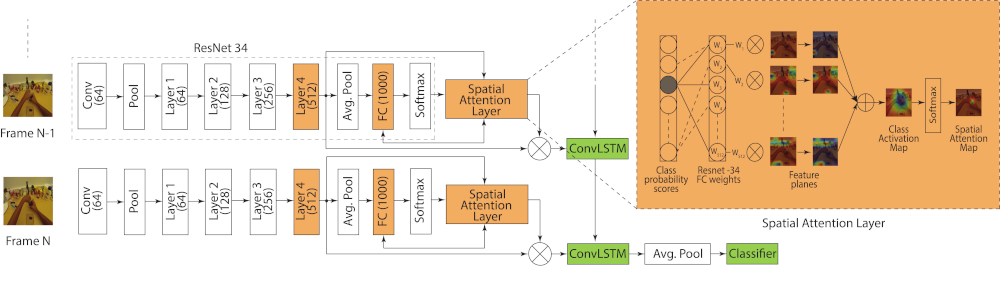
\includegraphics[width=\linewidth]{images/egornn.png}
	\caption{Architecture of \textit{egornn}}
	\label{egornn_arch}
\end{figure*}

\subsection{Flow\_resnet34}

\textit{Flow\_resnet34} is just a \textit{resnet34} edited to work with the warp flows. It gets five warp flows from \textit{processed\_frames\_x} and five from \textit{processed\_frames\_y} in form of a tensor of ten channels and tries to make predictions on the 61 classes.

\subsection{Two stream model}

Egornn learns appearence features, while \textit{flow\_resnet34} learns motion features. The way to join the two nets is to concatenate the two output layers and to add at the end a fully connected layer to get the class category scores.

\subsection{Motion Segmentation branch applied to egornn}

The problem which \cite{sparnet} tries to overcome is that in the two stream model motion and appearence are actually separately learned, without taking into account the spatial-temporal relationships.

We have built an architecture similar to \textit{sparnet}, where the \textit{motion segmentation block} is the same but the \textit{action recognition block} has been substituted by egornn (like in one of the attempts in \cite{sparnet}). The architecture is shown in \reff{msblock_arch}. We have used this architecture with some granular variations during our experiments, but the main blocks are always as shown in \reff{msblock_arch}. The input of the convolutional layer of MS Block is taken from one of the convolutional layers of \textit{resnet34} of egornn (the actual layer varies with our experiments). Then, after the convolutional layer, there is a fully connected layer followed by a softmax which normalizes the weights between 0 and 1. \textit{mmaps ground truth} and \textit{rgb ground truth} represent the mmaps and the rgb after the trasformations. The trasformations applied to the mmaps are the same applied to the rgbs, plus a small amount of proper mmaps trasformations which always ends with a trasformation which linearizes the pixels (from a 2 dimensional tensor per mmap we get a 1 dimensional tensor per mmap). For the msblock these linearized pixels represent a real ground truth, because each of the output neurons of the MS Block is used to predict the values of the mmaps ground truth. The pixel losses are summed together (obtaining as result $L_{ms}$) and then are summed again with the egornn loss ($L_c$). The final loss is used to compute the gradients to update the weights.

\begin{figure*}
	\centering
	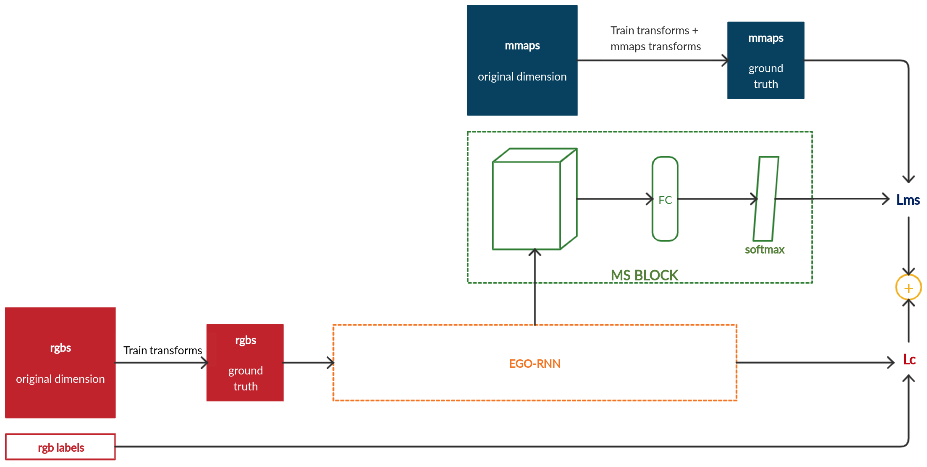
\includegraphics[width=\linewidth]{images/egornn+msblock_architecture.png}
	\caption{Generic architecture of motion segmentation branch applied to \textit{egornn}}
	\label{msblock_arch}
\end{figure*}

\section{Experiments}

\subsection{Egornn}

\subsection{Motion Segmentation branch applied to egornn}

% \subsection



{\small
\bibliographystyle{ieee}
\bibliography{egbib}
}

\end{document}
